\documentclass{article}
\usepackage{hyperref} 
\usepackage{graphicx} % Required for inserting images

\title{Solution Building Report}
\author{Hokimiyon Muhammadjon}
\date{November 2023}

\begin{document}

\maketitle

\section{Seq2Seq}
The task is the model take as input sentence than return as output the sentence.
The basic solution is Seq2Seq. The idea consist of encoder and decoder parts.
Encoder part take the input sentence, take their embedding and goes through rnn (gru).

Note: In the beginning prev\_hidden is zero.

The architecture of Encoder:

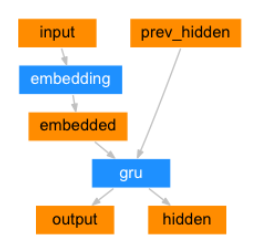
\includegraphics[scale=0.4]{figures/Encoder_seq2seq.png}

The Decoder part take the sentence input, then take embedding as in encoder part, activation function then rnn (gru) after takes softmax and the result goes to loss function.

Note: In the beginning prev\_hidden is the output of encoder part.

Note: input sentence have their behaviour in train and predict.

    In train input sentence is target sentence.

    In prediction, input sentence started with $<sos>$ (special symbol meaning start of sentence), and then step by step create sentence.

The architecture of Decoder part

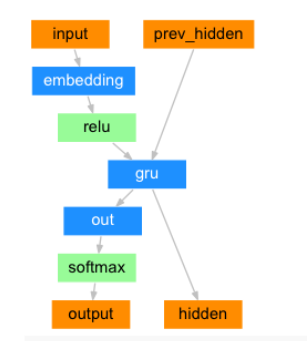
\includegraphics[scale=0.4]{figures/Decoder_seq2seq.png}


\section{Attention}
Attention architecture the same as seq2seq, except after gru layer in encoder and decoder goes multi-head attention layer.
In this algorithm encoder-decoder attention implemented.

The encoder-decoder attention calculates a weighted sum of the encoder's hidden states to create a context vector. This context vector is a dynamic representation of the relevant parts of the input sequence for generating the current output element. However, using a single attention mechanism can have limitations, such as not being able to focus on different aspects of the input sequence simultaneously. Multi-head attention addresses this limitation by using multiple sets of attention weights (heads) in parallel. Each head independently learns different attention patterns, allowing the model to focus on different parts of the input sequence for different aspects of the task

The attention layer architecture

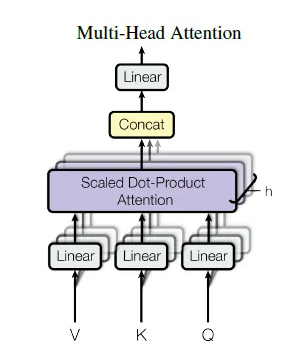
\includegraphics[scale=0.8]{figures/Attention_attentionblockpng.png}

\section{Transformer}
Transformer consist of encoder and decoder parts.

Encoder: The input sequence is fed into the encoder, which consists of multiple identical layers. Each layer has two main subcomponents: a multi-head self-attention mechanism and a feedforward neural network. The self-attention mechanism allows the model to consider different parts of the input sequence when encoding each element.

Decoder: The output sequence is generated by the decoder, which also consists of multiple identical layers. Each decoder layer combines self-attention and encoder-decoder attention mechanisms (as written in Attention section). The self-attention mechanism helps the decoder focus on different parts of the generated output sequence, while the encoder-decoder attention mechanism lets the model align the input and output sequences.

In transformer there is new part name Positional Encoding, because we don't use RNN type mechanism, we don't have information about positions, hence positional encodings are added to the input embeddings to provide the model with information about the position of each element in the sequence.

Also one more new part is feedforward Neural Networks: After applying attention mechanisms, each sublayer in the encoder and decoder includes a position-wise feedforward Neural Network to further process the information.

To stabilizing training and improving the flow of gradients through the deep network, the Layer Normalization and Residual Connections component introduced.

The architecture of Transformer:

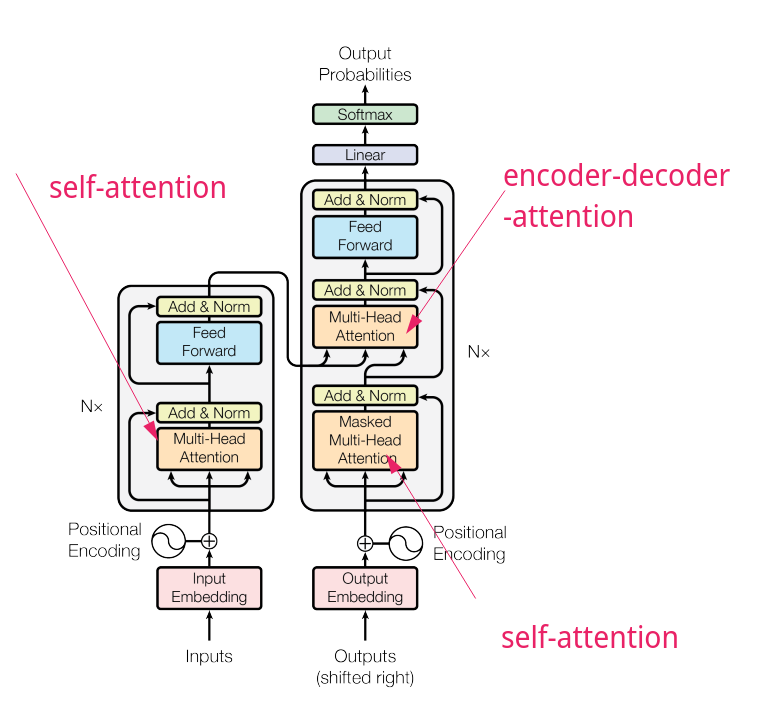
\includegraphics[scale=1]{figures/Transformer.png}

\section{Results}
\begin{itemize}
    \item origin $\mapsto$ original text
    \item translation $\mapsto$ translated text
    \item predicted $\mapsto$ the output of model
\end{itemize}

Seq2Seq:

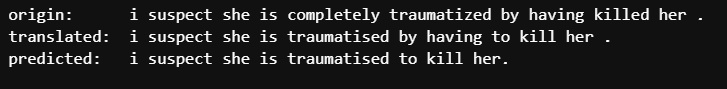
\includegraphics[scale=0.42]{figures/Seq2Seq_result_1.png}

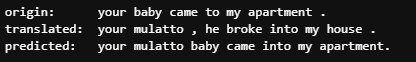
\includegraphics[scale=0.42]{figures/Seq2Seq_result_2.png}

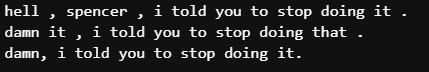
\includegraphics[scale=0.42]{figures/Seq2Seq_result_3.png}

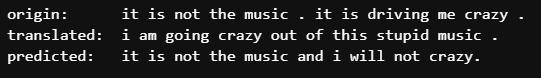
\includegraphics[scale=0.5]{figures/Seq2Seq_result_4.png}

Attention:

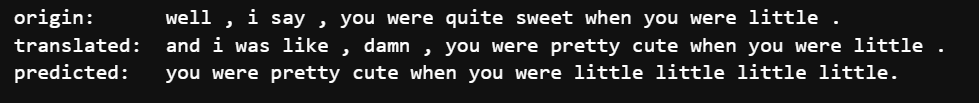
\includegraphics[scale=0.42]{figures/Attention_result_1.png}

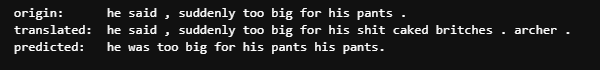
\includegraphics[scale=0.42]{figures/Attention_result_2.png}

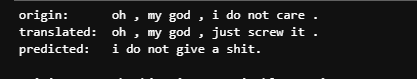
\includegraphics[scale=0.5]{figures/Attention_result_3.png}

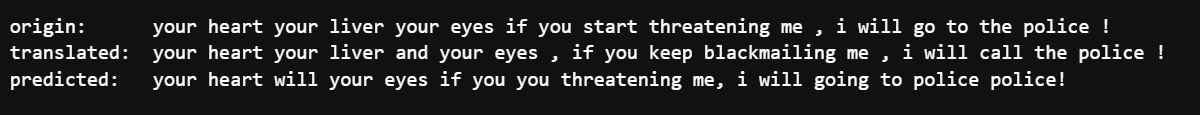
\includegraphics[scale=0.4]{figures/Attention_result_4.png}

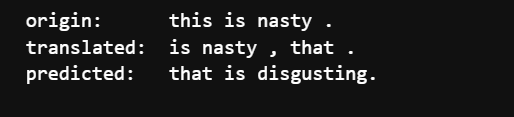
\includegraphics[scale=0.45]{figures/Attention_result_5.png}

Transformer:

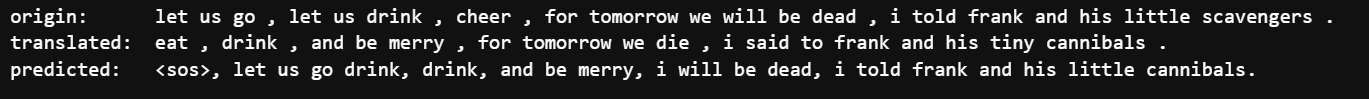
\includegraphics[scale=0.42]{figures/Transformer_result_1.png}

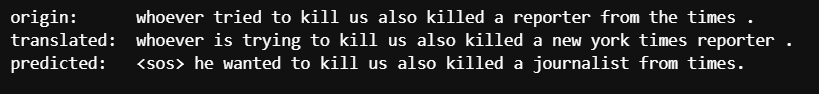
\includegraphics[scale=0.42]{figures/Transformer_result_2.png}

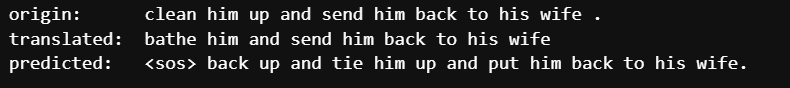
\includegraphics[scale=0.42]{figures/Transformer_result_3.png}

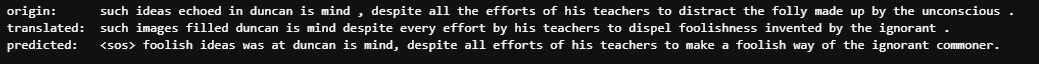
\includegraphics[scale=0.5]{figures/Transformer_result_4.png}

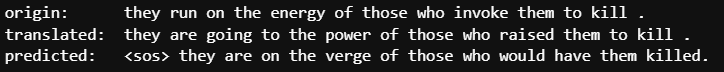
\includegraphics[scale=0.45]{figures/Transformer_result_5.png}

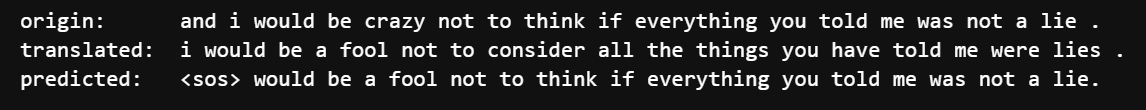
\includegraphics[scale=0.42]{figures/Transformer_result_6.png}

\begin{thebibliography}{2}
\bibitem{Seq2Seq}
Sean Robertson (2023) \emph{NLP From Scratch: Translation with a Sequence to Sequence Network and Attention}, Pytorch Tutorials. [\href{https://pytorch.org/tutorials/intermediate/seq2seq_translation_tutorial.html}{link}]

\bibitem{Transformer}
Vaswani, A. et al. (2017) \emph{Attention is All You Need}, In Advances in Neural Information Processing Systems, Vol. 30. [\href{https://papers.nips.cc/paper_files/paper/2017/hash/3f5ee243547dee91fbd053c1c4a845aa-Abstract.html}{link}]

\end{thebibliography}

\end{document}
